\chapter{让 IMU 预测，让激光纠偏}
\begin{notebox}
\textbf{目标}\quad 在同一时间轴上估计位置、速度、航向与偏置，理解预测和校正的分工。\\
\textbf{先修}\quad 第 06、08 章；本章逐步解释协方差和卡尔曼增益。
\end{notebox}

\section{先单独验证滤波器}
重新构建并加载工作区后，从仓库根目录运行：
\begin{lstlisting}[language=bash,numbers=none]
ros2 run motion2d planar_ekf_demo tmp/ch09_filter
/usr/bin/python3 scripts/plot_ch09_filter.py
\end{lstlisting}
先把两个问题分开：滤波器的矩阵是否正确，真实扫描匹配能否提供可靠观测？
这个实验只检查前者。位姿输入是从解析轨迹生成的带噪合成测量，\emph{不是激光 SLAM 验证}。
后续在线版本才使用第八章扫描匹配的实际输出。

IMU 给短时间运动变化；它并不知道初始速度或全局位置。
位姿观测虽然较慢，却可以修正累积误差，并通过时间关联帮助估计速度与偏置。
二者噪声模型不同，不能简单把两个位置取平均。

\section{八个数描述平面状态}
采用状态列向量
\begin{equation}
x=(p_x,p_y,v_x,v_y,\psi,b_{ax},b_{ay},b_g)^\top.
\end{equation}
$p,v$ 在 odom 系，$\psi$ 是航向；加计偏置 $b_a$ 在机体系，单位 m/s$^2$；
陀螺偏置 $b_g$ 单位 rad/s。原始 IMU 的 orientation 字段不参与计算。
因为机器人水平运动且 roll、pitch 为零，重力没有 x/y 分量：
\begin{equation}
a_k=R(\psi_k)(f_{xy,k}-b_{a,k}),\quad
\omega_k=\omega_{m,k}-b_{g,k}.
\end{equation}
对时长 $h$ 的一个小区间，用步首航向旋转并保持加速度，得到
\begin{equation}
\begin{aligned}
p_{k+1}&=p_k+h v_k+\tfrac12 h^2a_k, &v_{k+1}&=v_k+h a_k,\\
\psi_{k+1}&=\operatorname{wrap}(\psi_k+h\omega_k), &b_{k+1}&=b_k.
\end{aligned}
\end{equation}
这是离散近似：连续转动时，区间内的 $R$ 实际也在变化。
缩短步长可以减小该近似误差；不能把公式说成一般旋转运动的精确积分。
当前内核接受 $0<h\leq0.1$ s，长时间缺测应报告失效而不是一步越过。

\clearpage
\section{不确定性如何沿着状态传播}
协方差 $P$ 的对角项描述方差，非对角项描述两个误差的关联。
例如位置与速度相关后，一个位置校正也能改变速度。
令 $J=\left[\begin{smallmatrix}0&-1\\1&0\end{smallmatrix}\right]$，
$A_\psi=R(\psi)J(f_{xy}-b_a)$。状态转移雅可比中的几个关键块为
\begin{equation}
\begin{aligned}
F_{pv}&=hI,&F_{p\psi}&=\tfrac12h^2 A_\psi,&F_{v\psi}&=h A_\psi,\\
F_{pb_a}&=-\tfrac12h^2R,&F_{vb_a}&=-hR,&F_{\psi b_g}&=-h.
\end{aligned}
\end{equation}
剩余对角块为单位阵。下列真实源码同时构造一步状态、$F$ 和噪声输入雅可比 $G$：
\lstinputlisting[language=C++,linerange={imu_predict_begin-imu_predict_end},
  includerangemarker=false]{../ros2_ws/src/motion2d/src/estimation/imu_predictor.cpp}

设本次采样的测量方差为
$\Sigma_u=\operatorname{diag}(\sigma_{ax}^2,\sigma_{ay}^2,\sigma_g^2)$，则
\begin{equation}
P^-_{k+1}=F_kP^+_kF_k^\top+G_k\Sigma_u G_k^\top+Q_b.
\end{equation}
第六章配置的是\textbf{每采样}标准差，所以例如速度方差增量为 $h^2\sigma_a^2$，
位置与速度的互协方差增量为 $\tfrac12 h^3\sigma_a^2$。
不能直接套用连续白噪声密度的 $h\sigma_a^2$ 公式。

偏置固定零时，最后三个状态及其协方差保持零。
开启 estimate\_bias 后，偏置初始标准差默认为 $(.05,.05,.01)$；
另设随机游走标准差 $\sigma_b=(.0005,.0005,.0001)$，它们是每 $\sqrt{\rm s}$ 的量。
因此 $Q_b$ 只在偏置对角块添加 $h\operatorname{diag}(\sigma_b^2)$。
这描述缓慢变化的不确定性，不等于模拟器一定注入了随机游走。

\clearpage
\section{一次位姿校正为什么也能改变速度}
观测向量 $z=(p_x^{\rm obs},p_y^{\rm obs},\psi^{\rm obs})$，$H$ 只选择状态中的位置和航向。
创新、创新协方差与增益为
\begin{equation}
r=z-Hx^-,\qquad S=HP^-H^\top+R_z,\qquad K=P^-H^\top S^{-1}.
\end{equation}
$r$ 的航向分量必须用 wrap 归一化。例如预测 $179^\circ$、观测 $-179^\circ$，
应校正约 $2^\circ$，而非 $-358^\circ$。\textbf{练习 ch09-1} 补完 yaw\_residual.hpp；
程序检查跨界、多圈及恰好 $\pi$ 的边界。

代码使用线性方程求解，不显式求逆。先检查 $r^\top S^{-1}r\leq16.3$，
不满足则拒绝本次校正。门限只能检查观测与当前模型是否相容，无法判定哪一方一定正确。
若模型漏掉了真实偏置，过小的 $P$ 反而会让它拒绝正常观测。

接受时 $x^+=x^-+Kr$。为减少数值误差对协方差的破坏，采用 Joseph 形式：
\begin{equation}
P^+=(I-KH)P^-(I-KH)^\top+K R_z K^\top.
\end{equation}
\lstinputlisting[language=C++,linerange={ekf_correct_begin-ekf_correct_end},
  includerangemarker=false]{../ros2_ws/src/motion2d/src/estimation/planar_ekf.cpp}

$K$ 的速度、偏置行通常并不为零，因为此前预测已经建立了互协方差。
这就是只有位置/航向观测仍能间接校正其他状态的原因。没有运动变化或长期缺少外部观测时，
这些量也可能很难区分；算法不能凭空产生可观测性。

\begin{notebox}
\textbf{教学模型的边界}\quad 激光局部地图和当前估计共享历史，观测不是严格独立的。
固定 $R_z$ 也只是可解释的测量尺度。这里的 EKF 不宣称严格统计一致，
更不能用很小的协方差数字证明定位准确。
\end{notebox}

\section{偏置与一秒缺测实验}
合成轨迹为 $p=(\sin(0.6t),\;0.5[1-\cos(0.6t)])$ m、$\psi=0.6t$ rad。
使用 200 Hz IMU、10 Hz 位姿观测、20 s 时长，4 到 5 s 不提供位姿校正。
同一组噪声输入同时送给三个滤波器；seed=9090。
加计偏置为 $(.08,-.04)$ m/s$^2$，陀螺偏置为 $.01$ rad/s，滤波器没有收到这些答案。
初始速度先验为零、标准差 1 m/s；实际初速不为零，因此纯 IMU 还包含初速不可知的误差。

\clearpage
\begin{figure}[t]
\centering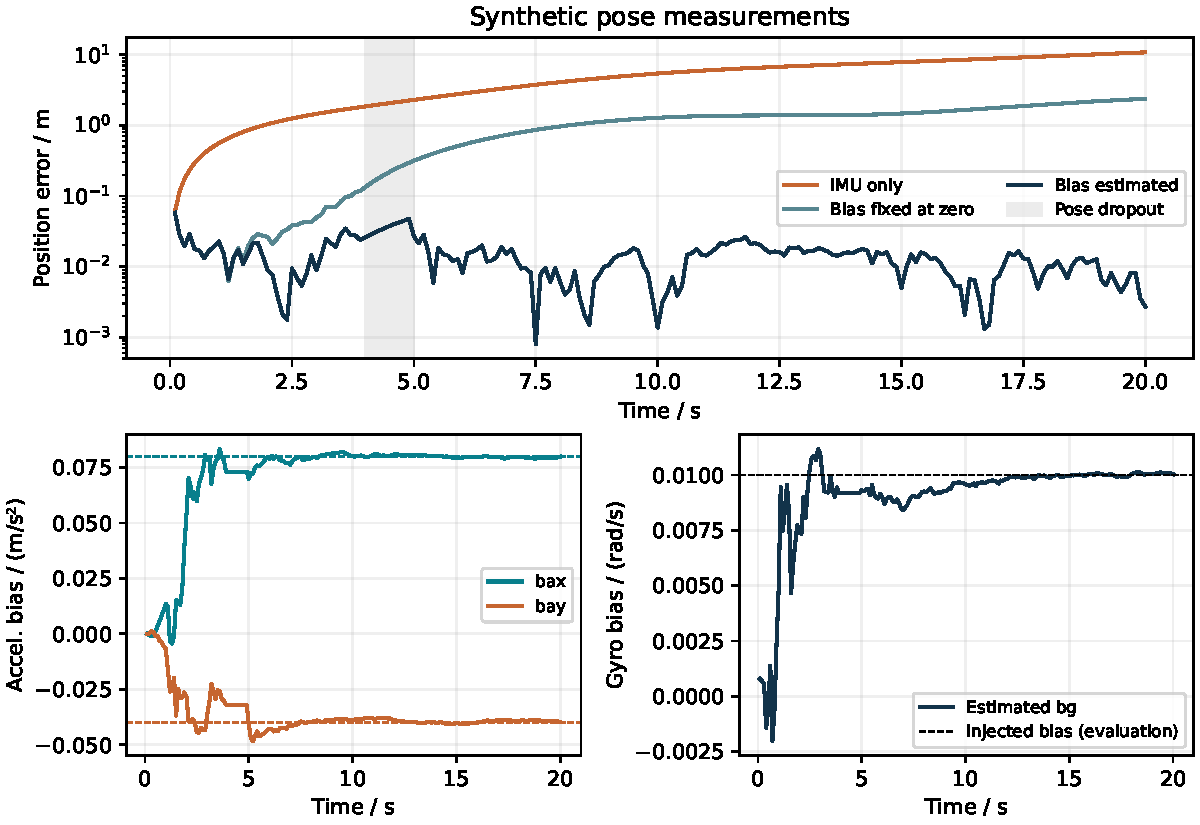
\includegraphics[width=\linewidth]{figures/ch09_filter.pdf}
\caption{合成位姿传感器实验。上图纵轴为对数，灰带表示停止位姿校正；下图虚线只用于评估注入的偏置。}
\end{figure}
\begin{center}\small
\pgfplotstabletypeset[col sep=comma,string type,
columns={mode,rmse,dropout_rmse,accepted,rejected},
columns/mode/.style={column name=模式,string replace*={imu_only}{仅 IMU},
  string replace*={fixed_zero_bias}{偏置固定零},string replace*={estimate_bias}{估计偏置}},
columns/rmse/.style={column name=全程 RMSE/m,fixed,precision=4,string type=false},
columns/dropout_rmse/.style={column name=缺测段 RMSE/m,fixed,precision=4,string type=false},
columns/accepted/.style={column name=接受},columns/rejected/.style={column name=拒绝},
every head row/.style={before row=\toprule,after row=\midrule},
every last row/.style={after row=\bottomrule}]{data/ch09_filter.csv}
\end{center}
表中误差统计全部 4000 个 IMU 时刻，接受/拒绝计数只针对低频位姿校正。
偏置固定零时，模型误差积累并触发大量拒绝；启用偏置估计后，本例全程位置 RMSE 约 0.0184 m。
这说明模型与置信度需要匹配，不意味着启用偏置状态在所有场景都更好。

\textbf{练习与验收：}手推 $F_{v\psi}$；完成角度残差练习；把注入偏置改为零后复跑，
再把观测标准差减半，比较误差及拒绝数。测试还核对常加速度解析解、$F/G$ 中心差分、
互协方差、离群点拒绝以及长时间更新后的协方差对称性与半正定性。
在线时间对齐将在下一个功能接入，不用合成观测实验冒充真实雷达定位。
